\documentclass[11pt,oneside]{amsart}
\usepackage{geometry}                % See geometry.pdf to learn the layout options. There are lots.
\geometry{letterpaper}                   % ... or a4paper or a5paper or ... 
%\geometry{landscape}                % Activate for for rotated page geometry
%\usepackage[parfill]{parskip}    % Activate to begin paragraphs with an empty line rather than an indent
\usepackage{graphicx}
\usepackage{amssymb}
\usepackage{amsmath}
\usepackage{comment}
\usepackage{epstopdf}
\usepackage{todonotes}
\DeclareGraphicsRule{.tif}{png}{.png}{`convert #1 `dirname #1`/`basename #1 .tif`.png}
\usepackage{wrapfig}
\usepackage{subfig}
%\usepackage[small,bf]{caption}
\graphicspath{{./Figures/}}            % Set path to folder for figures; relative path: folder "Figures" 

\title{Test Article}
%\author{The Author}
%\date{}                                           % Activate to display a given date or no date

\begin{document}
\maketitle
%\section{}
%\subsection{}


\begin{abstract}
The focus of this proposal is development of a new hybrid microfluidic/nanochannel method for realizing high-sensitivity, label-free biomolecular assays. The use of micro/nanofabrication enables the construction of multiple sensing modules, each having receptors attached for distinct analytes, all of which can sample the same, microliter-scale fluid specimen.
\end{abstract}


\section{My first section}
Here is a first line.
In essence, we take advantage of the desirable properties of microfluidics (mass production, manipulation of pL--$\mu$L volumes, reasonable pressures for flow, advection-based mass transport) in sample delivery, and then, after dynamic nanochannel formation, the small volume and high surface area are ideally suited for sensing measurement.\todo{Try out todo note} Thus, our approach combines the rapid response time attainable with transport in microfluidic channels with the enhanced sensitivity of nanochannel impedance measurement.\cite{Zou:2006wk}

\ensuremath{a = \frac{1}{x}}, $b = z^2_{max}$

\~n \^o

\subsection{And  a subsection} 

The focus of this proposal is development of a new hybrid microfluidic/nanochannel method for realizing high-sensitivity, label-free biomolecular assays.\footnote{Test footnote} The use of micro/nanofabrication enables the construction of multiple sensing modules, each having receptors attached for distinct analytes, all of which can sample the same, microliter-scale fluid specimen.

This method is thus scalable to multiplexed sensing of many analytes in the same microscale fluid volume, and thus addresses key limitations of existing approaches.\marginpar{Try out margin text} The proposed approach will utilize microfluidics for rapid sample transport, followed by dynamic formation of nanochannels for impedance-based sensing of the reduction in nanochannel volume due to target analyte binding to surface-attached receptors.\cite{Zhang:2011ft}

\begin{figure}[htb]
\centering
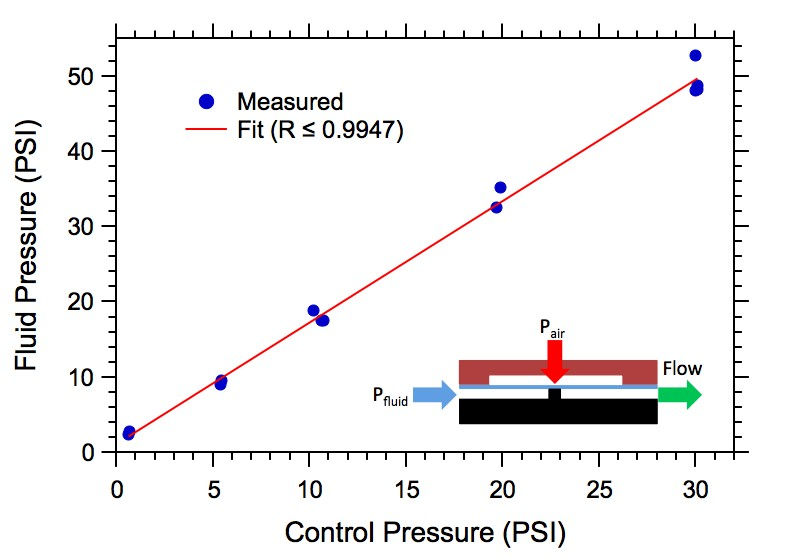
\includegraphics[width=0.8\textwidth]{20120102PEGValveDataLayout}
%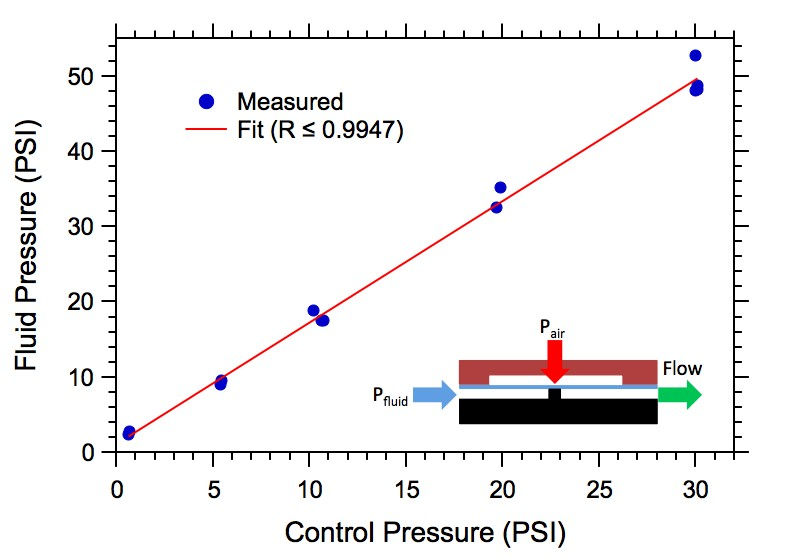
\includegraphics{20120102PEGValveDataLayout}
\caption{Awesome Image - my first one!}
\label{fig:awesome_image}
\end{figure}

\begin{figure}[htb]
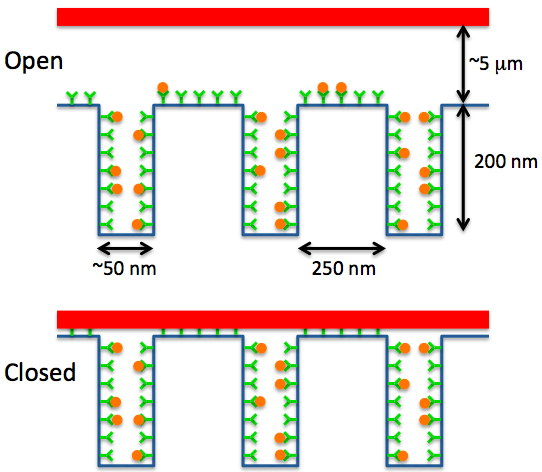
\includegraphics[width=0.5\textwidth]{PEGNanochannelSchematic}
\caption{Another awesome image.}
\label{fig:awesome_image}
\end{figure}

\begin{comment}This method is thus scalable to multiplexed sensing of many analytes in the same microscale fluid volume, and thus addresses key limitations of existing approaches.  The proposed approach will utilize microfluidics for rapid sample transport, followed by dynamic formation of nanochannels for impedance-based sensing of the reduction in nanochannel volume due to target analyte binding to surface-attached receptors. 
\end{comment}



In essence, we take advantage of the desirable properties of microfluidics (mass production, manipulation of pL--$\mu$L volumes, reasonable pressures for flow, advection-based mass transport) in sample delivery, and then, after dynamic nanochannel formation, the small volume and high surface area are ideally suited for sensing measurement. Thus, our approach combines the rapid response time attainable with transport in microfluidic channels with the enhanced sensitivity of nanochannel impedance measurement.\cite{Zhang:2011ft,Zou:2006wk,Yang:2010to}

Measurement results for a device fabricated in our cleanroom facilities are shown in Fig. 3(a), along with calculations based on the equivalent circuit model in Fig. 3(b). As seen in Fig. 3(a), for all frequencies parasitic capacitance (0.75 pF in our case) forms an upper bound on the magnitude of the impedance. When the flow channel is filled with phosphate buffered saline (PBS) solution (solid purple line) the impedance is dominated at low frequencies (<10 kHz) by double layer capacitance, Cdl, at the electrodes. Between 10 kHz and 1 MHz the solution impedance between the electrodes, Rsol, is dominant. When the PDMS valve is closed (red curve), the flat region between 1 kHz and 10 kHz is due to the nanochannel impedance, Rnc. Since it is substantially larger than the double layer capacitance and solution impedances, it is easily measureable. 

\subsubsection{A subsubsection}
The critical data is the measured impedance after exposure of the nanotrenches to bovine serum albumin (BSA) when BSA solution is driven through the flow channel while the PDMS valve is open. Since BSA non-specifically adheres to the flow channel surfaces, including the trench walls (the dissociation constant, $K_D$, is 200 nM), measurement with the PDMS valve closed shows a significant increase in impedance (blue curve) compared to the case of no protein adsorbed on the trench walls (red curve). The increase in impedance is large�a factor of 2.8. 

\begin{wrapfigure}{r}{0.5\textwidth}
  \begin{center}
    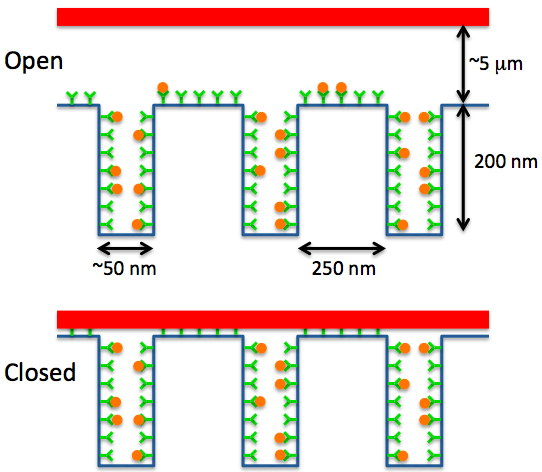
\includegraphics[width=0.48\textwidth]{PEGNanochannelSchematic}
  \end{center}
  \caption{Testing out having text flow around a figure.}
  \label{fig:wrapright1}
\end{wrapfigure}

Based on a Langmuir binding model for protein adsorption on nanochannel walls at equilibrium, we can estimate the minimum measurable protein concentration, cmin. The fraction of filled binding sites on the nanochannel walls, $\beta$, is $\alpha / (1 + \alpha )$ where $\alpha = (c / K_D)$ and $c$ is the analyte concentration. This gives the usual sigmoidal dose-response curve when $\beta$ is plotted on a linear y-axis against $\alpha$ on a log x-axis. At small concentrations relative to the dissociation constant (i.e., c<<KD), the fraction of filled binding sites is a linear function of $\alpha$, which we can rearrange as c = $\beta$KD. It is easy to show that the average nanochannel cross sectional area is a linear function of the fraction of filled binding sites on the nanochannel walls (starting, for example, with Eq. 4 of Ref. [50] and assuming a solution ion concentration similar to 1x PBS such that surface charge effects on impedance are negligible, which would be typical for actual measurement conditions). Since nanochannel impedance goes as the average nanochannel cross sectional area, the impedance is linearly related to the analyte concentration for c<<KD. One can therefore show that the minimum measurable protein concentration, cmin, goes as ?KD, where ? is the impedance measurement accuracy of our HP4294A impedance analyzer, which is 0.1\% if we can decrease the measured impedance to 100 k� or less. Using an antibody with KD = 1 nM (i.e., neither the best nor the worst available), this corresponds to cmin = ~2 pM. As an example, cardiac troponin T (cTnT) with a molar mass of 24 kDa would have a minimum measurable concentration of ~50 pg/mL. Use of averaging in conjunction with a comparative measurement should reduce this further to the sub pg/mL level, more than adequate sensitivity for cardiac biomarker measurement.

\begin{figure}[t]
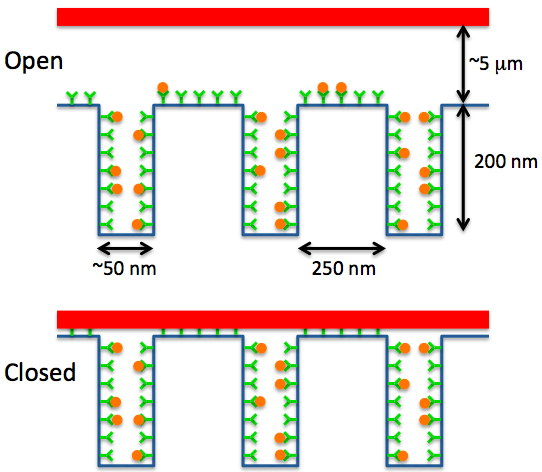
\includegraphics[width=0.4\textwidth]{PEGNanochannelSchematic}
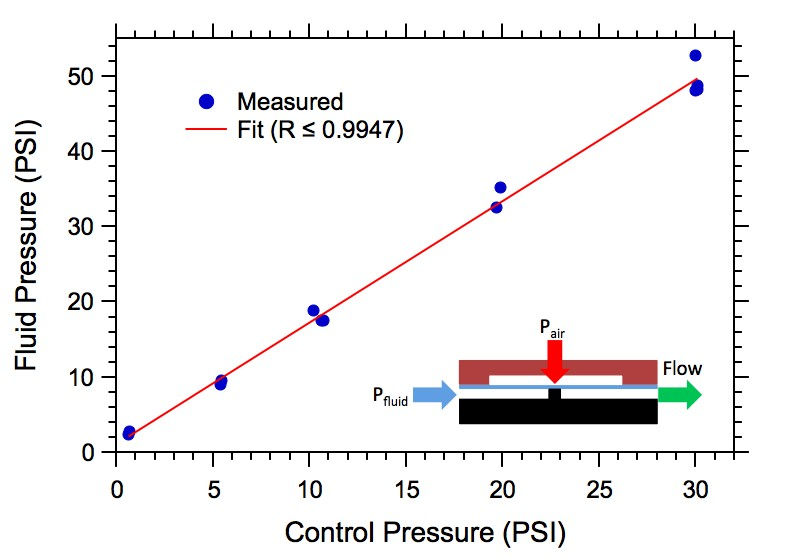
\includegraphics[width=0.4\textwidth]{20120102PEGValveDataLayout}
\caption{Another awesome image1.}
\label{fig:awesome_image1}
\end{figure}

\begin{figure}[b]
  \centering
  \subfloat[]{\label{fig:4a}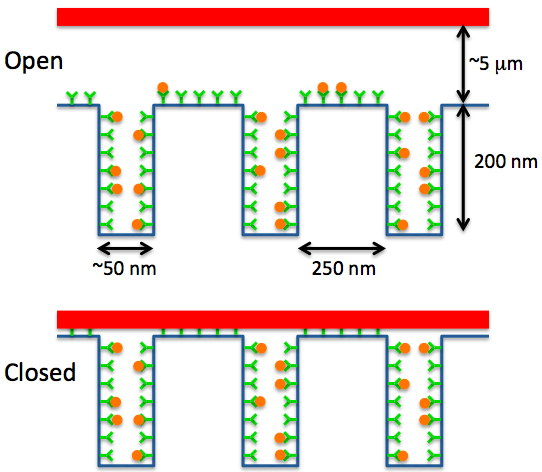
\includegraphics[width=0.4\textwidth]{PEGNanochannelSchematic}}
  \subfloat[]{\label{fig:4b}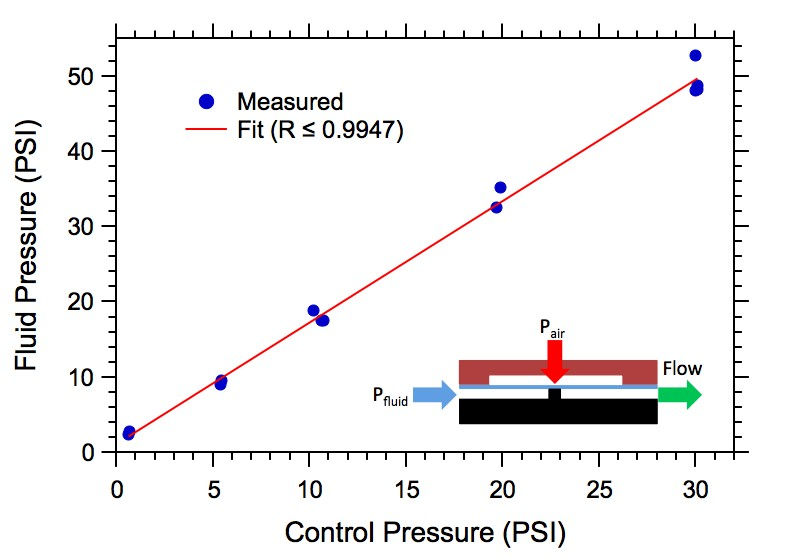
\includegraphics[width=0.4\textwidth]{20120102PEGValveDataLayout}}
  \caption{Another awesome image2.}
  \label{fig:awesome_image2}
\end{figure}

\subsubsection{Specific Aim 1 � Dynamic Nanochannel Optimization}
High sensitivity measurement of protein concentration with dynamic nanochannels requires high sensitivity measurement of impedance in conjunction with high receptor binding affinity. The greatest sensitivity for impedance measurement is obtained for impedances on the order of 100 k� or less. [63] To get into this range, a combination of criteria are needed: (1) short (~3 ?m or less) nanochannels, (2) many nanochannels in each array (100-1000), (3) higher aspect ratio nanotrenches, (4) reduced double layer capacitance (obtainable with surface treatment [64]), and (5) reduced solution resistance (larger electrodes set closer together). Our work with dynamic nanochannels using PDMS indicates that Criterion 1 (which is most critical) is highly challenging. After much effort, our shortest functional nanochannels are ~35 ?m, still an order of magnitude too long. We find that any attempt at further reduction in size is offset by trade-offs with flow constriction and channel collapse due to the overly flexible PDMS membranes. Consequently, we have developed new designs using poly-PEGDA valves for dynamic nanochannels, the fabrication and optimization of which are the focus of Specific Aim 1.

The approach we will pursue in this proposal is an adaptation of the poly-PEGDA valve geometry reported in Sect. 3.1.2 in which either nanotrenches (Fig. 5(a)) or shallow recesses (Fig. 5(b)) span the valve seat. When the valve membrane is actuated, it forms the top surface of nanochannels (for trenches) or nanogaps (for recesses). The bottom poly-PEGDA layer in Fig. 4(a) will be replaced with quartz to enable use of standard receptor attachment chemistries for the proof-of-principle studies in this proposal. Flow channels will be wet etched in the quartz, during which the valve seat can easily be made a few microns wide. Electrodes will be patterned in the bottom of the flow channels adjacent to the valve seat such that their separation will be only a few microns more than the valve seat width. Trenches will be etched in the top of the valve seat by FIB for rapid prototyping, or by electron-beam lithography and high aspect ratio plasma etching (with which Dr. Nordin�s group has many years experience [65-71]). Recesses will be wet etched. The upper poly-PEGDA layers will be bonded to the quartz through polymerization with a surface-attached silane containing an acrylate group. Details of the valve seat, flow channel, nanotrench and recess, and membrane geometry will be varied, guided by finite element simulation, to determine the combination of parameters that yields the highest sensitivity to protein concentration measurement. Optimal designs from simulation will be confirmed experimentally, first through comparison of the impedance in unmodified nanochannel arrays to that in the same channels after exposure to BSA, as in our preliminary results. Briefer adsorption times or lower BSA concentrations will be used to determine measurement sensitivity at lower analyte levels. Upon completion of this aim, we will have optimized dynamic nanochannel designs that provide discernable shifts in impedance after exposure to BSA levels as low as 1 ng/mL.

\bibliographystyle{ieeetr}
\bibliography{testBibTeX}
\end{document}  